  \documentclass[a4]{beamer}
\usepackage{amssymb}
\usepackage{graphicx}
\usepackage{subfigure}
\usepackage{newlfont}
\usepackage{amsmath,amsthm,amsfonts}
%\usepackage{beamerthemesplit}
%\usepackage{pgf,pgfarrows,pgfnodes,pgfautomata,pgfheaps,pgfshade}
\usepackage{mathptmx} % Font Family
\usepackage{helvet} % Font Family
\usepackage{color}
\mode<presentation> {
\usetheme{Default} % was Frankfurt
\useinnertheme{rounded}
\useoutertheme{infolines}
\usefonttheme{serif}
%\usecolortheme{wolverine}
% \usecolortheme{rose}
\usefonttheme{structurebold}
}
\setbeamercovered{dynamic}
\title[MA4413]{Statistics for Computing \\ {\normalsize MA4413 Lecture 5A/5B}}
\author[Kevin O'Brien]{Kevin O'Brien \\ {\scriptsize kevin.obrien@ul.ie}}
\date{Autumn 2013}
\institute[Maths \& Stats]{Dept. of Mathematics \& Statistics, \\ University \textit{of} Limerick}
\renewcommand{\arraystretch}{1.5}
%------------------------------------------------------------------------%
\begin{document}
\begin{frame}
\titlepage
\end{frame}
\begin{frame}
\frametitle{Lectures and Mid-Terms}
\begin{itemize}
\item Lecture Slot 5A was used for the first Mid-term exam.\\
\item The Lecture Series recommences in Lecture Slot 5B.
\item Lecture Slot 4B covered the Exponential Distribution. 
\item The next mid-term is provisionally scheduled take place in Week 9. The normal distribution, hypothesis testing (including the $t$-test), confidence intervals, and inference procedures are the only topics going to be examined in this mid-term.
\item Please be advised of sample papers for the second midterm in the SULIS directory.
\end{itemize}
\end{frame}
%------------------------------------------------------------%
\begin{frame}

\frametitle{Introduction to the Normal Distribution}
\begin{itemize}
\item
Recall the experiment whereby a die was rolled 100 times, and the sum of the 100 values was recorded.
\item
This experiment was repeated a very large number of times (e.g. 100,000 times ) in a simulation study.
\item
A histogram was drawn to depict the distribution of outcomes of this experiment.
\item Recall that we agreed that ``bell-shaped" was a good description of the histogram.

\end{itemize}
\end{frame}


\frame{
\frametitle{Normal Distribution}

\begin{center}
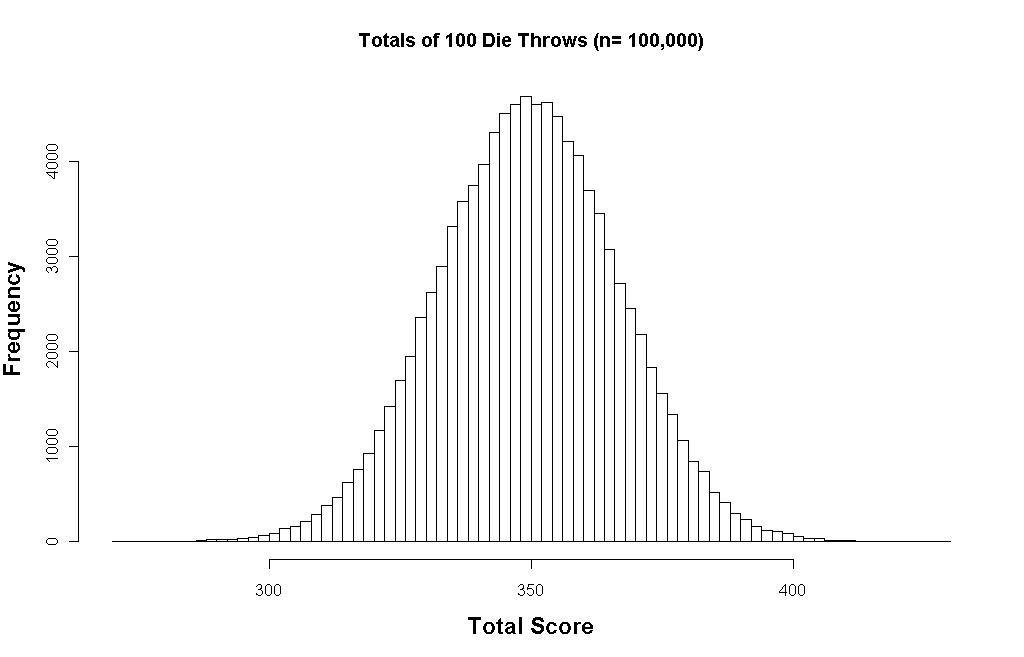
\includegraphics[scale=0.30]{3aDieHist3}
\end{center}

}
%----------------------------------------------------------------------%

\frame{
\frametitle{Normal Distribution}
\begin{itemize}
\item The normal distribution is perhaps the most widely used type of probability distribution for a random variable.
\item Normal distributions have the same general shape: the bell curve.
\item The distributions are \textbf{symmetric} with values concentrated more in the middle than in the tails.
%\item Examples of normal distributions are shown below. Notice that they differ in how spread out they are. The area under each curve is the same.
\item \alert{Important} The height of a normal distribution can be defined mathematically in terms of two fundamental parameters: the normal mean ($\mu$) and the normal
    standard deviation ($\sigma$).
\item A normally distributed random variable X is denoted $ X \sim \mbox{N} (\mu, \sigma^2)$ (note that we use the variance term here).
    \item The mean ($\mu$) and standard deviation ($\sigma$) are vital for calculating probabilities.
\end{itemize}
}
%------------------------------------------------------------------------%
\frame{
\frametitle{The Normal Distribution}
The \textbf{\emph{probability density function}} of the normal distribution is given as
\[ f(x) = \frac{1}{\sqrt{2\pi\sigma^2}} e^{ -\frac{(x-\mu)^2}{2\sigma^2} } \]

Integrating this formula would allow us to compute probabilities.


However, it is not required to use this formula.
}
%------------------------------------------------------------------%
\frame{
\frametitle{Normal Distribution}

\begin{center}
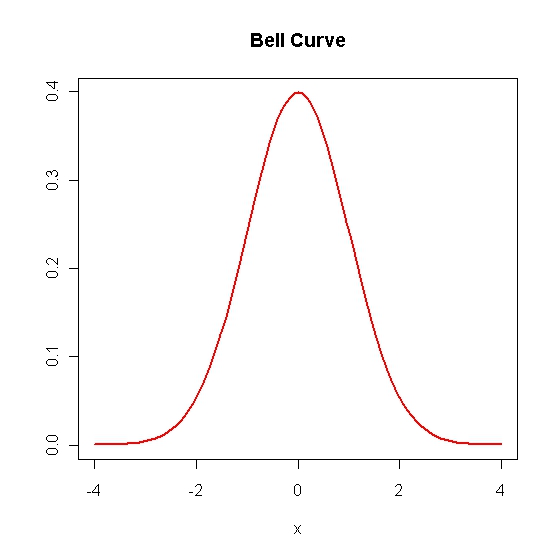
\includegraphics[scale=0.30]{5ABellCurve}
\end{center}

}
%------------------------------------------------------------------%
\frame{
\frametitle{Characteristics of the Normal probability distribution}
\begin{itemize}
\item[1] The highest point on the normal curve is at the mean, which is also the median of the distribution.
\item[2] \alert{[VERY IMPORTANT]}
The normal probability curve is bell-shaped and symmetric, with the shape of the curve to the left of the mean a mirror image of the shape of the curve to the right of the mean. (This is the basis of an important rule, called the \textbf{Symmetry Rule}, that we shall meet later.)
\item[3] The standard deviation determines the width of the curve. Larger values of the the standard deviation result in wider flatter curves, showing more dispersion in data.
\item[4] As with all density curves, the total area under the curve for the normal probability distribution is 1.
\end{itemize}
}
%------------------------------------------------------------------%
\frame{
\frametitle{ Characteristics of the Normal probability distribution}
\textbf{Remark:} It is useful to know the following statements as rules of thumb, but we will do all relevant calculations from first principles. However, in an exam situation, these rules of thumb may be invoked, and it is \textbf{NOT} required to show your workings.
\begin{itemize}
\item The interval defined by the mean $ \pm 1 \times $ standard deviation includes approximately $68\%$ of the observations, leaving $16\%$ (approx) in each tail.
\item The interval defined by the mean $ \pm 1.645 \times $ standard deviation includes approximately $90\%$ of the observations, leaving $5\%$ (approx) in each tail.
\item The interval defined by the mean $ \pm 1.96 \times $ standard deviation includes approximately $95\%$ of the observations, leaving $2.5\%$ (approx) in each tail.

\item The interval defined by the mean $ \pm 2.58 \times $ standard deviation includes approximately $99\%$ of the observations, leaving $0.5\%$ (approx) in each tail.
\end{itemize}

}
%------------------------------------------------------------------------%
\frame{
\frametitle{The Standard Normal Distribution}

\begin{itemize}

\item The standard normal distribution is a special case of the normal distribution with a mean $\mu= 0$ and a standard deviation $\sigma =1$.
\item We denote the standard normal random variable as $Z$ rather than $X$.
\[Z \sim N(0,1^2)\]
\item The distribution is well described in statistical tables (i.e. Murdoch Barnes Table 3, aka MB3)
\item Rather than computing probabilities from first principles, which is very difficult, probabilities from distributions other than the Z distribution (e.g. X $\sim$N($\mu=100, \sigma =15$)) can be computed using the Z distribution, a much easier approach. (We shall demonstrate how to do this shortly.)
\end{itemize}
}
%------------------------------------------------%
\frame{
\frametitle{Standardization formula}
All normally distributed random variables have corresponding $Z$ values, called \textbf{\emph{Z-scores}}.\\
\bigskip
For normally distributed random variables, the z-score can be found using the \textbf{\emph{standardization formula}};
\[z_o = { x_o - \mu \over \sigma}\]
where $x_o$ is a score from the underlying normal (``X") distribution, $\mu$ is the mean of the original normal distribution, and $\sigma$ is the standard deviation of original normal distribution.\\
\bigskip
Therefore $z_o$ is the z-score that corresponds to $x_o$.

\begin{itemize}
\item Terms with subscripts mean particular values, and are not variable names.
\item A computed Z-score is a normally distributed random variable only if the underlying distribution (X) is normally distributed. If the underlying distribution is not normal, then using Z-scores is not a valid approach.
\end{itemize}
}

%------------------------------------------------------------------------%
\frame{
\frametitle{The Standardized Value}
\Large
\begin{itemize}
\item Suppose that mean $\mu = 80 $ and that standard deviation $\sigma = 8$.
\item What is the Z-score for $x_o = 100$?
\[
z_{100} = {x_0 - \mu \over \sigma} = {100 - 80 \over 8} = {20 \over 8} = 2.5
\]
\item Therefore the Z score is : $z_{100} = 2.5$
\end{itemize}
}
%------------------------------------------------------------------------%
\frame{
\frametitle{Z-scores}
\begin{itemize}
\item A Z-score always reflects the number of standard deviations above or below the mean a particular score is.
\item 
Suppose the scores of a test are normally distributed with a mean of 50 and a standard deviation of 9
\item For instance, if a person scored a 68 on a test, then they scored 2 standard deviations above the mean.

\item Converting the test scores to z scores, an X value of 68 would yield:
\[ Z = {68 - 50 \over 9} =2 \]

\item So, a Z score of 2 means the original score was 2 standard deviations above the mean.
\end{itemize}

}
%------------------------------------------------------------------------%
%\end{document}
% The standardization formula
% used to find Z values

%

%------------------------------------------------------------------------%
\frame{
\frametitle{The Standard Normal (Z) Distribution Tables}
\begin{itemize}
\item Importantly, probabilities relating to the z distribution are comprehensively tabulated in \textbf{\emph{Murdoch Barnes Table 3}}.
\item This is available on sulis, in the ``about this module" folder.
\item Given a value of $k$ (with k usually between 0 and 4), the probability of a standard normal ``Z" random variable being greater than (or equal to) k $P(Z \geq k)$ is given in Murdoch Barnes table 3 .
\item Other statistical tables can be used (e.g. the Dept. of Education Tables that many student would have used in school), but they may tabulate probabilities in a different way.
\end{itemize}
}

%------------------------------------------------------------------------%
\frame{
\frametitle{An Important Identity}
If two values $z_o$ and $x_o$ are related in the following way, for some values $\mu$ and $\sigma$,
\[
z_{0} = {x_0 - \mu \over \sigma}
\]
Then we can can say

\[ P(X \geq x_o) = P(Z \geq z_o) \]

or alternatively

\[ P(X \leq x_o) = P(Z \leq z_o) \]

This is fundamental to solving problems involving normal distributions.

}

%------------------------------------------------------------------------%
\frame{
\frametitle{Using Murdoch Barnes Tables 3}
\begin{itemize}
\item For some value $z_o$, between 0 and 4, the Murdoch Barnes tables set 3 tabulate $P(Z \geq z_o)$
\item Ideally $z_o$ would be specified to 2 decimal places. If it is not, round to the closest value.
\item We call the third digit (i.e. the digit in the second decimal place) the ``second precision".
\end{itemize}
}

%------------------------------------------------------------------------%
\frame{
\frametitle{Using Murdoch Barnes Tables 3}
\begin{itemize}
\item To compute the relevant probability we express $z_o$ as the sum of $z_o$ without the second precision, and the second precision.(For example $1.28 = 1.2 + 0.08$.)
\item Select the row that corresponds to $z_o$ without the second precision (e.g. 1.2).
\item Select the column that corresponds to the second precision(e.g. 0.08).
\item The value that contained on the intersection is $P(Z \geq z_o)$
\end{itemize}
}

%------------------------------------------------------------------------%
\frame{
\begin{table}[ht]
\frametitle{Find $ P(Z \geq 1.28)$}
\vspace{-1.5cm}
%\caption{Standard Normal Distribution } % title of Table
\centering % used for centering table
\begin{tabular}{|c|| c c c c c c|} % centered columns (4 columns)
\hline %inserts double horizontal lines
& \ldots & \ldots & 0.006 &0.07&0.08&0.09 \\
%heading
\hline \hline% inserts single horizontal line
\ldots & \ldots & \ldots &\ldots& \ldots &\ldots&\dots \\ % inserting body of the table
1.0 & \ldots & \ldots &0.1446& 0.1423 &0.1401&0.1379 \\ % inserting body of the table
1.1 & \ldots & \ldots&0.1230& 0.1210 &0.1190&0.1170 \\ % inserting body of the table
1.2 & \ldots & \ldots&0.1038 & 0.1020 &\alert{0.1003}&0.0985\\
1.3 & \ldots & \ldots &0.0869& 0.0853 &0.0838&0.0823 \\ % inserting body of the table
\ldots & \ldots &\ldots&\ldots & \ldots &\ldots&\ldots\\
\hline %inserts single line
\end{tabular}
%\label{table:nonlin} % is used to refer this table in the text
\end{table}
}

%------------------------------------------------------------------------%
\frame{
\frametitle{Using Murdoch Barnes tables 3}
\begin{itemize}
\item Find $ P(Z \geq 0.60)$
\item Find $ P(Z \geq 1.64)$
\item Find $ P(Z \geq 1.65)$
\item Estimate $P( Z \geq 1.645)$
\end{itemize}
}

%------------------------------------------------------------------------%
\frame{
\begin{table}[ht]
\frametitle{Find $ P(Z \geq 0.60)$}
\vspace{-1.5cm}
%\caption{Standard Normal Distribution } % title of Table
\centering % used for centering table
\begin{tabular}{|c|| c c c c c c|} % centered columns (4 columns)
\hline %inserts double horizontal lines
& 0.00 & 0.01 & 0.02 &0.03&\ldots&\ldots \\
%heading
\hline \hline% inserts single horizontal line \hline
\ldots & \ldots &\ldots &\ldots& \ldots &\ldots&\ldots \\ % inserting body of the table
0.4 & 0.3446 & 0.3409&0.3372 & 0.3336 &\ldots&\ldots\\
0.5 & 0.3085 & 0.3050 &0.3015& 0.2981 &\ldots&\dots \\ % inserting body of the table
0.6 & \alert{0.2743} & 0.2709&0.2676 & 0.2643 &\ldots&\ldots\\
0.7 & 0.2420 & 0.2389 &0.2358& 0.2327 &\ldots&\dots \\ % inserting body of the table
\ldots & \ldots &\ldots &\ldots& \ldots &\ldots&\ldots \\ % inserting body of the table
\hline %inserts single line
\end{tabular}
%\label{table:nonlin} % is used to refer this table in the text
\end{table}
}

%------------------------------------------------------------------------%
\frame{
\begin{table}[ht]
\frametitle{Find $ P(Z \geq 1.64)$ and $ P(Z \geq 1.65)$}
\vspace{-1.5cm}
%\caption{Standard Normal Distribution } % title of Table
\centering % used for centering table
\begin{tabular}{|c|| c c c c c c|} % centered columns (4 columns)
\hline %inserts double horizontal lines
& \ldots & \ldots & 0.04 & 0.05 &0.06&0.07 \\
%heading
\hline \hline% inserts single horizontal line
\ldots & \ldots &\ldots &\ldots& \ldots &\ldots&\ldots \\ %Checked
1.5 & \ldots & 0.0630&0.0618& 0.0606 &0.0594&\dots \\ % inserting body of the table
1.6 & \ldots &0.0516& \alert{0.0505} & \alert{0.0495} &0.0485&\ldots\\
1.7 & \ldots &0.0418 &0.0409& 0.0401 &0.0392&\dots \\ % inserting body of the table
\ldots & \ldots &\ldots &\ldots& \ldots &\ldots&\ldots \\ %Checked
\hline %inserts single line
\end{tabular}
%\label{table:nonlin} % is used to refer this table in the text
\end{table}
}

%------------------------------------------------------------------------%
\frame{
\frametitle{Using Murdoch Barnes tables 3}
\begin{itemize}
\item $ P(Z \geq 1.64) = 0.505$
\item $ P(Z \geq 1.65) = 0.495$ \bigskip
\item $ P(Z \geq 1.645)$ is approximately the average value of $ P(Z \geq 1.64)$ and $ P(Z \geq 1.65)$.
\item $ P(Z \geq 1.645)$ = (0.0495 + 0.0505)/2 = 0.0500. ( i.e. $5\%$ )
\end{itemize}
}
%------------------------------------------------------------------%
\frame{
\frametitle{Exact Probability}
\large
\alert{Remarks:} This is for continuous distributions only.
\begin{itemize}
\item The probability that a continuous random variable will take an exact value is infinitely small.
We will usually treat it as if it was zero.
\item
When we write probabilities for continuous random variables in mathematical notation, we often retain the equality component (i.e. the "...or equal to..").\\
For example, we would write expressions $P(X \leq 2)$ or $P(X \geq 5)$.
\item
Because the probability of an exact value is almost zero, these two expression are equivalent to $P(X < 2)$
or $P(X > 5)$. \item The complement of $P(X \geq k)$ can be written as $P(X \leq k)$.
\end{itemize}
}


%------------------------------------------------------------------%
\frame{
\frametitle{Complement and Symmetry Rules}

Any normal distribution problem can be solved with some combination of the following rules.
\begin{itemize} \item \textbf{Complement rule} \item Common to all continuous random variables
\[P(Z \geq k) = 1 - P(Z \leq k) \]
Similarly
\[P(X \geq k) = 1 - P(X \leq k) \]
\end{itemize}

\[P(Z \leq 1.28) = 1 - P(Z \geq 1.28)  = 1-0.1003 = 0.8997\]
}

%------------------------------------------------------------------%
\frame{
\frametitle{Complement and Symmetry Rules}
\begin{itemize}
\item \textbf{Symmetry rule}
\item
This rule is based on the property of symmetry mentioned previously.
\item
Only the probabilities corresponding to values between 0 and 4 are tabulated in Murdoch Barnes.
\item
If we have a negative value of k, we can use the symmetry rule.
\end{itemize}
\[P(Z \leq -k) = P(Z \geq k) \]
by extension, we can say
\[P(Z \geq -k) = P(Z \leq k) \]
}
%------------------------------------------------------------------%
\frame{
\frametitle{Z Scores: Example 1 }
Find $P(Z \geq -1.28)$\\
\textbf{Solution}\\
\begin{itemize}
\item Using the symmetry rule
\[P(Z \geq -1.28) = P(Z \leq 1.28) \]
\item Using the complement rule
\[P(Z \geq -1.28) = 1 - P(Z \geq 1.28) \]
\[P(Z \geq -1.28) = 1 - 0.1003 = 0.8997 \]
\end{itemize}
}
%------------------------------------------------------------------%
\frame{
\frametitle{Z Scores: Example 2 }
Find the probability of a Z random variable being between -1.8 and 1.96?
i.e. Compute $P(-1.8 \leq Z \leq 1.96)$\\
Solution
\begin{itemize}
\item Consider the complement event of being in this interval: a combination of being too low or too high.
\item
The probability of being too low for this interval is $P(Z \leq -1.80) = 0.0359$ (check)
\item
The probability of being too high for this interval is $P(Z \geq 1.96) = 0.0250$ (check)
\item
Therefore the probability of being \textbf{outside} the interval is 0.0359 + 0.0250 = 0.0609.
\item
Therefore the probability of being \textbf{inside} the interval is 1- 0.0609 = 0.9391
\[P(-1.8 \leq Z \leq 1.96) = 0.9391\]
\end{itemize}
}





%--------------------------------------------------------------
\begin{frame}
\frametitle{Application : Example }
The mean time spent waiting by customers before their queries are dealt with at an information centre is 10 minutes.

The waiting time is normally distributed with a standard deviation of 3 minutes.
\begin{itemize}
\item [i)] What percentage of customers will be waiting longer than 15 minutes

\item [ii)] $90\%$ of customers will be dealt with in at most 12 minutes. Is this statement true or false?
Justify your answer.

\item [iii)] What percentage of customers will wait between 7 and 13 minutes before their query is dealt with?
\end{itemize}
\end{frame}
%---------------------------------------------%
\begin{frame}
\frametitle{Solutions}

Let x be the normal random variable describing waiting times\\
$P(X \geq 15) =?$ \\
\bigskip
     First , we find the z-value that corresponds to x = 15  (remember $\mu=10$ and $\sigma=3$  )\\
\[ z_o = { x_o - \mu \over \sigma }  = { 15 - 10 \over 3 } = 1.666 \]
\begin{itemize}
\item We will use $z_o =1.67$
\item Therefore we can say $P(X \geq 15 ) = P(Z \geq 1.67)$
\item The Murdoch Barnes tables are tabulated to give $P(Z \geq z_o)$ for some value $ z_o$ .
\item We can evaluate $P(Z \geq 1.67)$  as 0.0475.
\item Necessarily $P(X \geq 15) = 0.0475$.
\end{itemize}
\end{frame}

%---------------------------------------------%
\begin{frame}
\frametitle{Solutions}
\begin{itemize}
\item "$90\%$ of customers will be dealt with in at most 12 minutes."
\item To answer this question, we need to know  $P(X\leq 12)$
\item First , we find the z-value that corresponds to x = 12  (remember $\mu=10$ and $\sigma=3$ )
\end{itemize}
\[ z_o = { x_o - \mu \over \sigma }  = { 12 - 10 \over 3 } = 0.666 \]

\end{frame}

%---------------------------------------------%
\begin{frame}
\frametitle{Solutions}
\begin{itemize}
\item We will use $z_o =0.67$ (although 0.66 would be fine too) 
\item Therefore we can say $P(X \geq 12 ) = P(Z \geq 0.67)  = 0.2514$
\item Necessarily  $P(X \leq 12 ) = P(Z \leq 0.67) = 0.7486$
\item $74.86\%$ of customers will be dealt with in at most 12 minutes.
\item The statement that $90\%$ will be dealt with in at most 12 minutes is false.
\end{itemize}
\end{frame}
%---------------------------------------------%
\begin{frame}
\frametitle{Solutions}
What percentage will wait between 7 and 13 minutes ?\\

$P(7 \leq X \leq 13)   = ?$

\textbf{Solution:}\\
Compute the probability of being too low, and the probability of being too high for the interval.\\The probability of being inside the interval is the complement of the combination of these events.
\end{frame}
%---------------------------------------------%
\begin{frame}
\frametitle{Solutions}
\textbf{Too high:}\\
$P(X \geq 13) = ?$
\[ z_o  = {13 - 10  \over 3} = 1\]

From tables, $P(Z \geq 1) = 0.1587$. Therefore $P(X \geq 13) = 0.1587$\\ \bigskip
\textbf{Too low:}\\
$P(X \leq 7) = ?$
\[ z_o  = {7 - 10  \over 3} = -1\]
By symmetry, and using tables, $P(X \leq 7) = P(Z \leq -1)= 0.1587$\\ \bigskip
\end{frame}
%---------------------------------------------%
\begin{frame}
\frametitle{Solutions}

\[P(7 \leq X \leq 13)  = 1 - [ P(X \leq 7)  + P(X \geq 13) ] \]

\[P(7 \leq X \leq 13)  =  1 - [0.1587+0.1587] = 0.6826\]

\end{frame}

%-----------------------------------------------------%
\begin{frame}
\frametitle{Normal Distribution : Solving problems}
Recap:
\begin{itemize}
\item We must know the normal mean $\mu$ and the normal standard deviation $\sigma$.
\item The normal random variable is $X \sim \mbox{N} ( \mu , \sigma^2)$.
\item (If we don't, we usually have to determine them, given the information in the question.)
\item The standard normal random variable is $Z\sim \mbox{N} ( 0 , 1^2)$.
\item The standard normal distribution is well described in Murdoch Barnes Table 3, which tabulates $P(Z \geq z_o)$ for a range of $Z$ values.
\end{itemize}
\end{frame}
%-----------------------------------------------------%
\begin{frame}
\frametitle{Normal Distribution : Solving problems}
\begin{itemize}
\item For the given value $x_o$ from the variable $X$, we compute the corresponding z-score $z_o$.
\[ z_o = { x_o - \mu \over \sigma} \]
\item When $z_o$ corresponds to $x_o$, the following identity applies:
\[  P(X \geq x_o )= P(Z \geq z_o ) \]
\item Alternatively $ P(X \leq x_o )= P(Z \leq z_o ) $
\end{itemize}
\end{frame}
%-----------------------------------------------------%
\begin{frame}
\frametitle{Normal Distribution : Solving problems}
\begin{itemize}
\item \textbf{Complement Rule}: \[ P(Z \leq k) = 1-P(Z \geq k) \] for some value $k$
\item Alternatively $ P(Z \geq k) = 1-P(Z \leq k) $
\item \textbf{Symmetry Rule}: \[ P(Z \leq -k) = P(Z \geq k) \] for some value $k$
\item Alternatively $ P(Z \geq -k) = P(Z \leq k) $
\end{itemize}
\end{frame}
%-----------------------------------------------------%
\begin{frame}
\frametitle{Normal Distribution : Solving problems}
\begin{itemize}

\item \textbf{Intervals}: \[ P(L \leq Z \leq U) = 1- [ P(Z \leq L) + P(Z \geq U)] \]
where $L$ and $U$ are the lower and upper bounds of an interval.
\item Probability of having a value too low for the interval : $P(Z \leq L)$
\item Probability of having a value too high for the interval : $P(Z \geq U)$
\end{itemize}
\end{frame}
%-----------------------------------------------------%


%\frame{
%\frametitle{Using Murdoch Barnes Tables 3}
%
%Find $ P(Z \geq 1.64)$ and $ P(Z \geq 1.65)$.\\\bigskip Which row and column?
%\begin{itemize}
%\item 1.64 = \color{blue}{1.6}+\color{orange}{0.04} \color{black}\hspace{2cm}$ P(Z \geq 1.64) =0.0505$
%\item 1.65 = \color{blue}{1.6}+\color{green}{0.05}  \color{black} \hspace{2cm}$ P(Z \geq 1.65) =0.0495$
%\end{itemize}
%\bigskip
%\small
%\begin{table}[ht]
%%\caption{Standard Normal Distribution } % title of Table
%\centering % used for centering table
%\begin{tabular}{|c|| c c c c c c|} % centered columns (4 columns)
%\hline %inserts double horizontal lines
%& & \ldots & \color{orange}{0.04} & \color{green}{0.05} &0.06&0.07\ldots \\
%%heading
%\hline \hline% inserts single horizontal line
%\ldots & \ldots &\ldots &\ldots& \ldots &\ldots&\ldots \\ %Checked
%1.5 & \ldots & 0.0630&0.0618& 0.0606 &0.0594&\dots \\ % inserting body of the table
%\color{blue}{1.6} & \ldots &0.0516& \alert{0.0505} & \alert{0.0495} &0.0485&\ldots\\
%1.7 & \ldots &0.0418 &0.0409& 0.0401 &0.0392&\dots \\ % inserting body of the table
%\ldots & \ldots &\ldots &\ldots& \ldots &\ldots&\ldots \\ %Checked
%\hline %inserts single line
%\end{tabular}
%%\label{table:nonlin} % is used to refer this table in the text
%\end{table}
%}

%--------------------------------------------------------%

%------------------------------------------------------------%
\begin{frame}

\frametitle{Normal Distribution: Simulation Study}
\begin{itemize}
\item
Recall the experiment whereby a die was rolled 100 times, and the sum of the 100 values was recorded.
\item
This experiment was repeated a very large number of times (e.g. 100,000 times ) in a simulation study.
\item
A histogram was drawn to depict the distribution of outcomes of this experiment.


\end{itemize}
\end{frame}


\frame{
\frametitle{Normal Distribution: Simulation Study}

\begin{center}
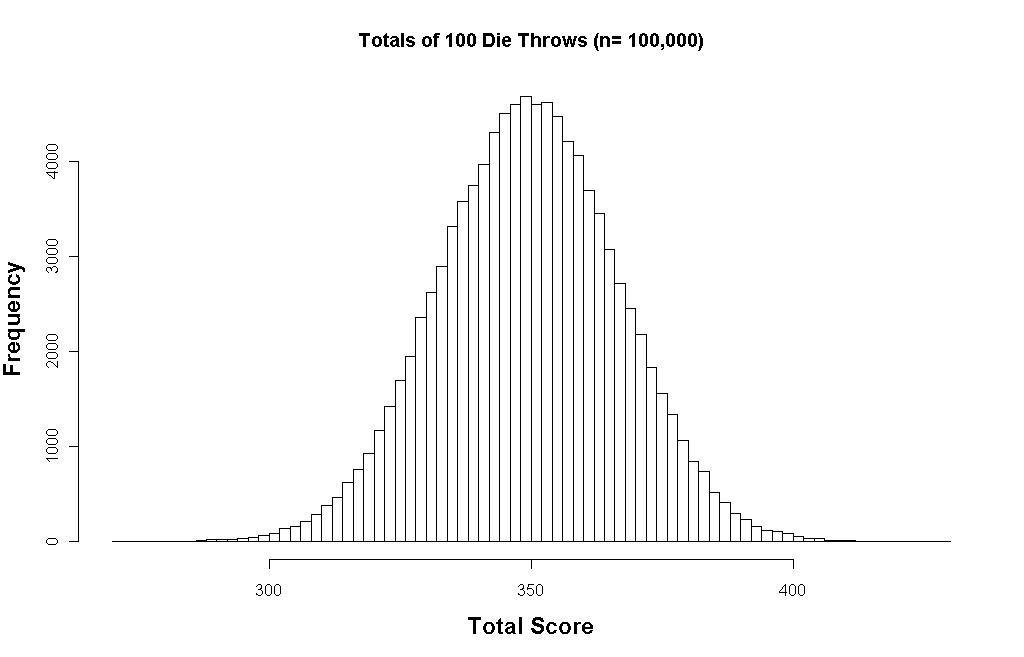
\includegraphics[scale=0.30]{3aDieHist3}
\end{center}

}

\frame{
\frametitle{Normal Distribution: Simulation Study}
Recall some observations made about the results of the simulation study, made in a previous lecture.
\begin{itemize}
% \item Approximately 76\% of the values are between 330 and 370.
\item Approximately 68.7\% of the values in the simulation study are between 332 and 367.
\item Approximately 95\% of the values are between 316 and 383.
\item $2.5\%$ of the values output are less than 316.
\item $2.5\%$ of the values study output are greater than 383.
\item 175 values are greater than or equal to 400, whereas 198 values are less than or equal to 300.
\item Results such as these are unusual, but they are not impossible.
\end{itemize}
}
%---------------------------------------------------------------%
\frame{
\frametitle{Normal Distribution: Simulation Study}
\begin{itemize}
\item Suppose we can \textbf{\emph{approximate}} the summation of the die-throws using the normal distribution.
\item The normal mean is necessarily $\mu = 350$.
\item The normal standard deviation is approximately 17. (68\% of values between $350 \pm 17$).
\item Using the normal distribution, lets estimate the proportion of values greater than 383.
\end{itemize}
}

%---------------------------------------------------------------%
\frame{
\frametitle{Normal Distribution: Simulation Study}

\begin{center}
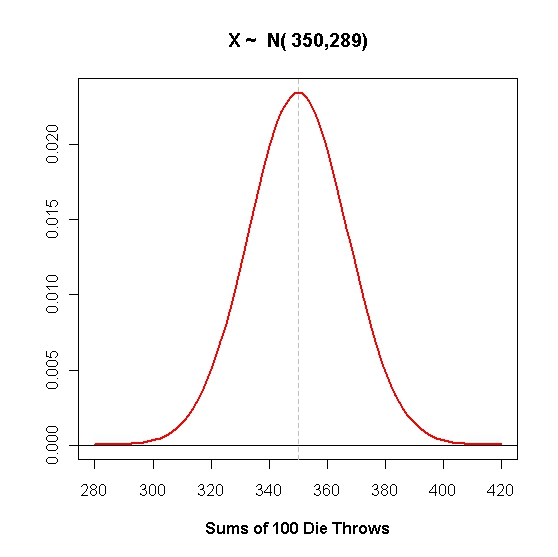
\includegraphics[scale=0.40]{5BNormalA}
\end{center}
}

%-------------------------------------------------------------%
\frame{
\frametitle{Normal Distribution: Simulation Study}
\begin{itemize}
\item X is the normal random variable that approximates the sum of values from 100 throws of a die.
\item Find $P(X \leq 383)$
\item First use the standardization formula to find the Z-score.
\[ z_o = {383 - 350 \over 17} = {33 \over 17} = 1.94 \]
\item Use the tables to compute $P(Z \geq 1.94)$ (\alert{Answer: 0.0262} )
\item Because $P(Z \geq 1.94)  = 0.0262$, we can say $P(X \geq 383)  = 0.0262$
\item This is close to the proportion of observed values, which was 2.5\%.
\item Remark : The standard deviation of 17 was an estimate. The actual standard deviation should 17.12.
\end{itemize}
}

\frame{
\frametitle{Normal Distribution: Simulation Study}

\begin{center}
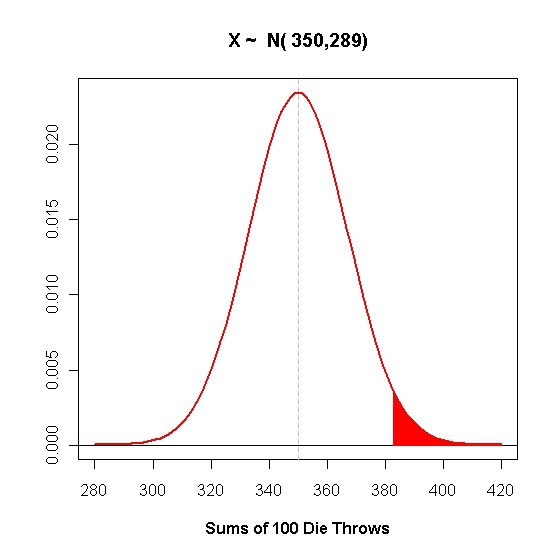
\includegraphics[scale=0.40]{5BNormalB}
\end{center}

}
%-------------------------------------------------------------%
\frame{
\frametitle{Working Backwards}
\begin{itemize}

\item Suppose we wish to find a value (lets call it A) from the normal distribution, such that a certain proportion of values is greater than A (e.g. 10\%)
\item Find A such that $P(X \geq A) = 0.10$. (with $\mu  = 350$ and $\sigma = 17$)
\item In general, our first step is to use the standardization equation to find the corresponding Z-score $z_A$.
\item Because we don't know what value A has, we can't use this approach.
\item However, we can say the following
\[  P(X \geq A) = P(Z \geq z_A) = 0.10 \]

\item From the tables, we can approximate a value for $z_A$, by finding the closest probability value, and determining the corresponding Z-score.
\end{itemize}
}

%------------------------------------------------------------------------%
\frame{

\frametitle{Find $z_A$ such that $ P(Z \geq z_a) = 0.10$}
\begin{itemize}
\item The closest probability value in the tables is $0.1003$.\\
\item The Z-score that corresponds to $0.1003$ is 1.28.\\
\item (Row : 1.2 , Column : 0.08)
\item Therefore $z_A  \approx 1.28$
\end{itemize}
\small
\begin{table}[ht]
%\caption{Standard Normal Distribution } % title of Table
\centering % used for centering table
\begin{tabular}{|c|| c c c c c c|} % centered columns (4 columns)
\hline %inserts double horizontal lines
& \ldots & \ldots & 0.006 &0.07&0.08&0.09 \\
%heading
\hline \hline% inserts single horizontal line
\ldots & \ldots & \ldots &\ldots& \ldots &\ldots&\dots \\ % inserting body of the table
1.0 & \ldots & \ldots &0.1446& 0.1423 &0.1401&0.1379 \\ % inserting body of the table
1.1 & \ldots & \ldots&0.1230& 0.1210 &0.1190&0.1170 \\ % inserting body of the table
1.2 & \ldots & \ldots&0.1038 & 0.1020 &\alert{0.1003}&0.0985\\
1.3 & \ldots & \ldots &0.0869& 0.0853 &0.0838&0.0823 \\ % inserting body of the table
\ldots & \ldots &\ldots&\ldots & \ldots &\ldots&\ldots\\
\hline %inserts single line
\end{tabular}
%\label{table:nonlin} % is used to refer this table in the text
\end{table}
}
%-------------------------------------------------------------%
\frame{
\frametitle{Working Backwards}
\begin{itemize}
\item We can now use the standardization formula.
\item We have only one unknown in the formula: $A$.
\[ 1.28 = {A - 350 \over 17} \]
\item Re-arranging ( multiply both sides by 17):\\
$ 21.76 = A - 350 $
\item Re-arranging ( add 350 to both sides ):\\
$ A = 371.76 $
\item $P(X \geq 371.76) \approx 0.10$
\item (Remark: for sums of die-throws, round it to nearest value)
\end{itemize}
}
%-----------------------------------------------------%

%-------------------------------------------------------------%
\frame{
\frametitle{Working Backwards: Another Example}
\begin{itemize}

\item Find B such that $P(X \geq B) = 0.90$. (with $\mu  = 350$ and $\sigma = 17$)
\item Necessarily $P(X \leq B) = 0.10$
\item Find some value $Z_B$ such that $P(Z \leq z_B) = 0.10$
\item $z_B$ could be negative.
\item Use the symmetry rule $P(Z \leq z_B) = P(Z \geq -z_B)$
\item $-z_B$ could be positive.
\item Based on last example $-z_B = 1.28$. Therefore $z_B = -1.28$
\end{itemize}
}
%-------------------------------------------------------------%
\frame{
\frametitle{Working Backwards}
\begin{itemize}
\item Again ,we can now use the standardization formula
\item We have only one unknown in the formula: $B$.
\[ -1.28 = {B - 350 \over 17} \]
\item Re-arranging ( multiply both sides by 17):\\
$ -21.76 = B - 350 $
\item Re-arranging ( add 350 to both sides ):\\
$ x_o = 350 - 21.76 = 328.24 $
\item $P(X \leq 328.24) \approx 0.10$
\end{itemize}
}
%-----------------------------------------------------%



\frame{
\frametitle{MA4413 Autumn 2008 paper}
A model of an on-line computer system gives a mean times to retrieve a record from a direct access storage system device of 200 milliseconds, with a standard deviation of 58 milliseconds. If it can assumed that the retrieval times are normally distributed:

\begin{itemize}
\item[(i)] What proportion of retrieval times will be greater than 75 milliseconds?
\item[(ii)] What proportion of retrieval times will be between 150 and 250 milliseconds?
\item[(iii)] What is the retrieval time below which 10\% of retrieval times will be?
\end{itemize}

}
%---------------------------------------------%

\frame{
\frametitle{Normal Distribution}

\begin{center}
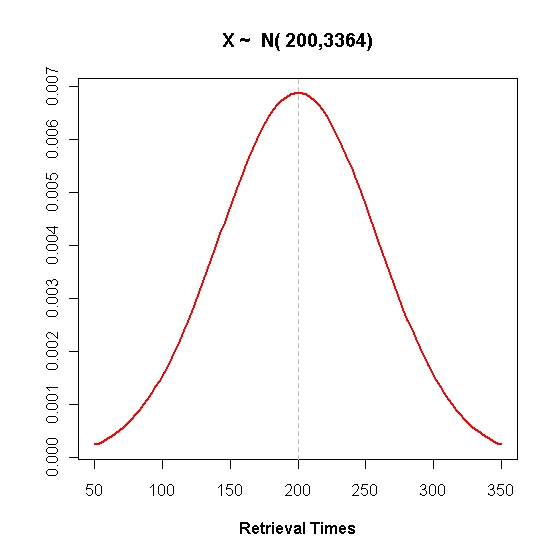
\includegraphics[scale=0.40]{5BNormal1}
\end{center}

}
%-----------------------------------------------------%


\frame{
\frametitle{MA4413 Autumn 2008 paper (part 1)}
What proportion of retrieval times will be greater than 75 milliseconds?\\ \bigskip

\begin{itemize}
\item Let X be the retrieval times, with $X \sim \mbox{N}(200,58^2)$.\\
\item The first question asks us to find $P( X \geq 75)$. \\
\item First compute the z score.
\[ z_o =  {x_o - \mu \over \sigma} = {75 - 200 \over 58}  = -2.15 \]
\end{itemize}
}

\frame{
\frametitle{Normal Distribution}

\begin{center}
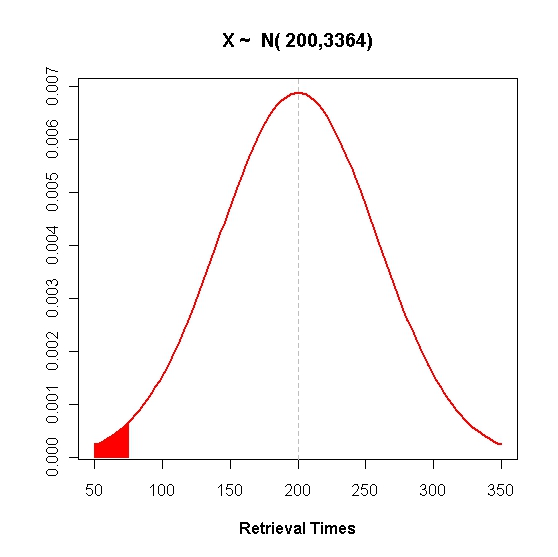
\includegraphics[scale=0.40]{5BNormal2}
\end{center}

In this case, the probability of interest $P(X\geq 75)$, is represented by the white area under the curve.

}

\frame{
\frametitle{MA4413 Autumn 2008 paper (part 1)}
\begin{itemize}
\item We can say
\[ P( X \geq 75) = P( Z \geq -2.15)\]
\item Using symmetry rule and complement rule
\[ P( Z \geq -2.15) = P( Z \leq 2.15) = 1- P( Z \geq 2.15)\]
\item From tables $P( Z \geq 2.15) = 0.0158$
\item Therefore $P( Z \leq 2.15) = 0.9842$
\item Furthermore $P( X \geq 75) = \boldsymbol{0.9842}$ [Answer].
\end{itemize}
}
\frame{
\frametitle{Normal Distribution}

\begin{center}
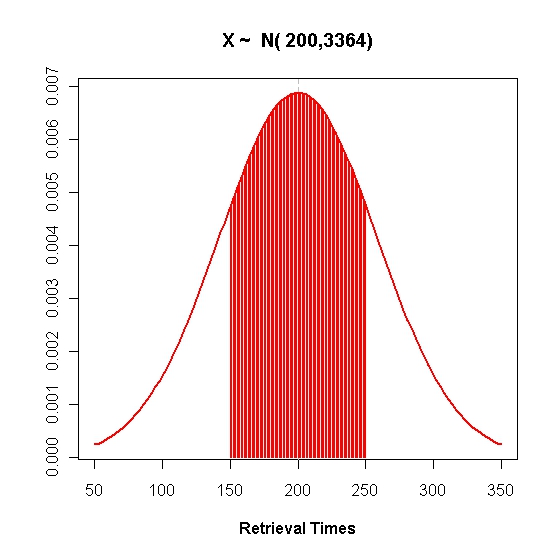
\includegraphics[scale=0.40]{5BNormal3}
\end{center}

}
%---------------------------------------------%
\frame{
\frametitle{MA4413 Autumn 2008 paper (part 2)}
\begin{itemize}
\item What proportion of retrieval times will be between 150 and 250 milliseconds?
\item Find $P(150 \leq X \leq 250)$
\item Use the `Too Low / Too High ' approach.
\item Too low $P( X \leq 150)$
\item Too high $P( X \geq 250)$
\item Find the z-scores for each.
\[ z_{150} =  {150 - 200 \over 58}  = -0.86 \]
\[ z_{250} =  {250 - 200 \over 58}  = 0.86 \]
\end{itemize}
}
%---------------------------------------------%
\frame{
\frametitle{MA4413 Autumn 2008 paper (part 2)}
\begin{itemize}
\item We can now say
\[ 1. P( X \leq 150) = P( Z \leq -0.86)\]
\[ 2. P( X \geq 250) = P( Z \geq 0.86)\]
\item By symmetry rule, $P( Z \leq -0.86) = P( Z \geq 0.86)$
\[ P( X \leq 150) =  P( X \geq 250) \]
\item Let's compute $P( X \geq 250)$. Using tables
\[P( X \geq 250) = P( Z \geq 0.86) = 0.1949 \]
\end{itemize}
}
%---------------------------------------------%
\frame{
\frametitle{MA4413 Autumn 2008 paper (part 2)}
\begin{itemize}
\item Too high: $P( X \geq 250) = 0.1949 $
\item Too low:  $P( X \leq 150) = 0.1949 $
\item Probability of being inside interval:

\[ P(150 \leq X \leq 250) = 1- [ P( X \leq 150) + P( X \geq 250)] \]

\item $P(150 \leq X \leq 250) = 1- [ 0.1949 + 0.1949 ] = \boldsymbol{0.6102}$

\end{itemize}
}
%---------------------------------------------%
\frame{
\frametitle{MA4413 Autumn 2008 paper (part 3)}
\begin{itemize}
\item What is the retrieval time below which 10\% of retrieval times will be?
\item Find $A$ such that $P(X \leq A) = 0.10$.
\item What z-score would correspond to $A$? Lets call it $z_A$.
\item $P(Z  \leq z_A) = 0.10$
\item Remark: $z_A$ could be negative.
\item Using symmetry $P(Z \geq -z_A) = 0.10$
\item Remark: $-z_A$ could be positive.
\end{itemize}
}

\frame{
\frametitle{Normal Distribution}

\begin{center}
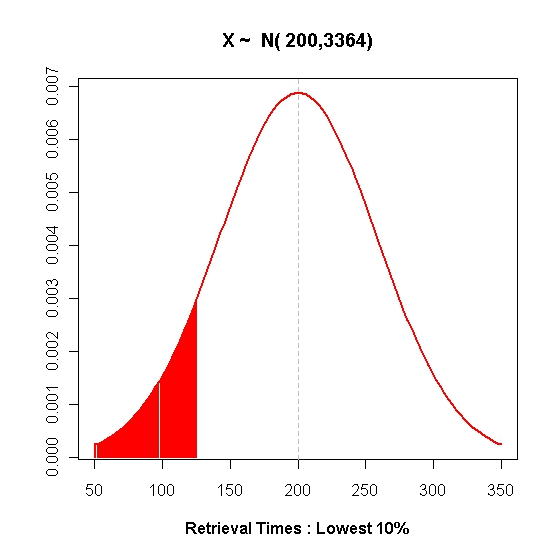
\includegraphics[scale=0.40]{5BNormal4}
\end{center}

}
%---------------------------------------------%
\frame{
\frametitle{MA4413 Autumn 2008 paper (part 3)}
\begin{itemize}
\item Use the Murdoch Barnes tables to get an approximate value for $-z_A$.
\item The nearest value we can get is 1.28. ( $P( Z \geq 1.28) = 0.1003$ ).
\item If $-z_A = 1.28$, then $z_A=-1.28$
\item We can now say
\[ P(X \leq A) = P(Z \leq -1.28) \]

\end{itemize}
}
%---------------------------------------------%
\frame{
\frametitle{MA4413 Autumn 2008 paper (part 3)}
\begin{itemize}
\item Necessarily $A$ and $Z_A$ are related by the standardization formula
\item Recall that $\mu = 200$ and $\sigma = 58$.
\[ -1.28  = {A - 200 \over 58} \]
\item Re-arranging ( multiply both sides by 58)
\[ -74.24  = A - 200 \]
\item Re-arranging again (Add 200 to both sides)
\[ 125.76 =  A \]
\end{itemize}
}
%---------------------------------------------%
\frame{
\frametitle{MA4413 Autumn 2008 paper (part 3)}
\begin{itemize}
\item Now we know the retrieval time below which 10\% of retrieval times will be.
\item $P(X \leq 125.76) = 0.10$ [Answer].
\end{itemize}
}
%---------------------------------------------%
\end{document} 